\chapter{Mapping the Industry: A Quantitative Analysis of DPP Initiatives}
\label{cha:chapter_3}

This chapter undertakes an empirical exploration of the \acrlong{dpp} industry development landscape by analyzing existing initiatives. Drawing on the publicly available dataset compiled by the CIRPASS project, the chapter seeks to provide a high-level quantitative assessment of how \ac{dpp}-related efforts are distributed across regions, industries, scope and more \autocite{CIRPASS.2024}. The results illuminate current trends and possible gaps in the adoption of \ac{dpp} solutions, thereby offering a contextual foundation for the system modeling and pilot implementation that follow in \Cref{cha:chapter_4} and \Cref{cha:chapter_5}.

To achieve these goals, the chapter starts with describing the initiatives dataset and the rationale for selecting it, elaborating on how it underpins the present research questions. (\Cref{sec:dataset_overview}) It continues to explain the data cleaning and preprocessing procedures undertaken to ensure consistent, reliable results. (\Cref{sec:data_cleaning_preprocessing}) Building on these preparations, the last section presents an exploratory data analysis, highlighting descriptive statistics and technology co-occurrence patterns. (\Cref{sec:data_analysis}) Taken together, these empirical findings reinforce or challenge the assumptions derived from the theoretical foundations in \Cref{cha:chapter_2}, thus sharpening the focus for the practical work detailed in later chapters.

\section{Dataset Overview}
\label{sec:dataset_overview}
As part of this empirical exploration, this study utilizes the publicly accessible \ac{dpp}-Related Initiatives Dataset compiled by the CIRPASS project. CIRPASS, a consortium aimed at fostering interoperability and widespread adoption of \ac{dpp}s, has curated a data repository of global efforts, including industry consortia, pilot programs, and start-ups, that engage with \ac{dpp} concepts. In view of its breadth and the diversity of entries, this dataset offers a vantage point from which to map the existing \ac{dpp} landscape and identify patterns in technological, organizational, and geographical focus. \autocite{CIRPASS.2024}

A preliminary inspection of the CIRPASS dataset shows a total of 205 recorded initiatives, each capturing metadata across 44 columns. While the majority of these columns store descriptive fields (e.g., "Initiative name", "Sector", "Technology readiness") as string values (\verb|object| dtype), a small number are classified as numeric (\verb|float64| dtype), typically containing missing or placeholder entries rather than genuine numerical data.

A high-level check confirms that several core features, like "Sector", "Host organization name", and "Technology readiness", among others, are populated for most entries, ensuring each project can be reliably identified and assigned a broad category. Conversely, some specialized columns (e.g., "Website", "Relevance", and "Label", "Certification", "Compliance") remain largely or entirely unpopulated, indicating that more advanced or company-specific information was not consistently reported by initiative providers.

Despite these occasional data gaps, the dataset remains sufficiently comprehensive for an exploratory assessment of key patterns, such as the types of technology deployed, the industries involved, and the general maturity of \ac{dpp} solutions. Fields like Solution type (e.g., “Platform,” “Traceability Solution”) and Market scope (e.g., “International,” “EU,” or “National”) further provide a lens into the functional and geographic breadth of each initiative. Alongside this, textual descriptors in columns like "Goal / USP / Benefit" offer a qualitative sense of project motivations and objectives, albeit with varying degrees of detail.

Overall, while certain attributes (such as "Relevance") appear sparsely filled, the presence of consistently populated fields (e.g., "Initiative name", "Sector", "Technology readiness") indicates that the dataset is well suited to a high-level quantitative mapping of the \ac{dpp} landscape. The subsequent \Cref{sec:data_cleaning_preprocessing} will address any minor inconsistencies and missing values to enable a robust exploratory analysis.

\section{Data Cleaning and Preprocessing}
\label{sec:data_cleaning_preprocessing}

A first step involved reducing the dataset to a set of columns deemed most relevant for the present analysis. In particular, fields such as "Initiative name", "Sector", "Solution type", and "Technology readiness" were retained for their direct usefulness in mapping the \ac{dpp} landscape across industry domains and development stages. Additionally, several columns capturing product-level data (e.g., "Product traceability", "Functional" and "technical specifications", "Data use management") were preserved for examining how initiatives address key lifecycle metrics. Columns found to be largely empty, redundant, or outside the scope of this research were omitted to streamline subsequent processing and visualization tasks. After this filtering, 205 records remained, each described by 37 variables; a compact yet sufficiently descriptive subset of the CIRPASS dataset for exploring \ac{dpp} adoption patterns.

After narrowing the dataset to the most relevant columns, the next step addressed missing data. An initial scan revealed that certain fields, especially "Goal / USP / Benefit", "Solution type", "Sector", and "Host organization type", were critical for distinguishing initiative characteristics yet contained some incomplete entries. Given their importance, these columns were imputed with a placeholder value (“Unknown”), ensuring that essential segmentation and categorization remained feasible. A similar procedure was applied to columns with moderate missingness: textual fields were imputed with “Unknown,” while any numerical fields (though few in number) were filled with the median to preserve distributional properties. By applying straightforward yet consistent imputation rules rather than discarding partially complete records, the dataset retained its original sample size of 205 entries, thus maximizing representativeness while mitigating potential bias.

Subsequently, the column headers were standardized to ensure consistency and clarity across the dataset, replacing the original textual labels (such as “Potential for cross-sectors application ?”) with more succinct, underscore-separated names (e.g., “Potential\_Cross\_Sector”). This renaming step was undertaken to facilitate more streamlined referencing in the subsequent analysis and to uphold best practices for data management, particularly when integrating the dataset with additional scripts or libraries.

Before proceeding with detailed cleaning, a dedicated preprocessing pipeline was established to ensure that the raw data is transformed into a consistent and analyzable form. This pipeline comprises several custom functions:

\begin{itemize}[itemsep=0.5\baselineskip]
    \item \verb|clean_text|: Removes extraneous non-alphanumeric characters (while preserving spaces and commas) and standardizes text to lowercase, thereby preparing free-text fields for uniform keyword matching.

    \item \verb|normalize_and_split_smart|: Splits multi-valued entries on commas while preserving content within parentheses, ensuring that each element is correctly identified even when additional clarifications are provided.
    
    \item \verb|standardize_values| and \verb|apply_partial_match|: These functions consolidate variant expressions by mapping them to standardized labels, reducing noise from spelling or phrasing inconsistencies.
    
    \item \textbf{Binary normalization functions}: Convert affirmative and negative responses into consistent “yes” and “no” values across binary columns.
\end{itemize}

This modular pipeline was engineered as a solid foundation for the subsequent cleaning process, facilitating robust downstream analyses by ensuring that both textual and categorical data are harmonized.

Finally, the pipeline was executed on the dataset. First, free-text fields, such as "Goal\_USP\_Benefit" were cleaned of extraneous characters and set to lowercase (see \verb|clean_text|) to ensure uniformity in later keyword matching or visualizations. Additionally, columns allowing multiple entries (e.g., "Sector", "Solution\_Type") were split on commas while preserving text within parentheses, a custom procedure that mitigates misclassification whenever items include follow-up clarifying descriptors. This multi-valued approach (via \verb|normalize_and_split_smart|) enabled downstream calculations on how frequently each discrete label (e.g., “platform,” “traceability solution,” “cross-sector”) appeared within a single cell.

Afterwards, a standardization step aligned differing textual variants, such as “cross-sector (more than one)” to simply “cross-sector”, and consolidated semantically equivalent tokens based on partial rule matching (e.g., “data scheme” → “product data scheme”). This systematic mapping clarified the range of unique categories and reduced noise caused by variations in spelling or phrasing. Several binary indicators (such as "Machine\_Readable\_Data\_Carrier") were then normalized, converting any affirmative text (e.g., “Yes,” “y,” “true,” or “1”) to a single “yes,” and similarly grouping all negative variations to “no.” Lastly, for each multi-valued field, an additional column counted the number of entries in the resulting list, supporting subsequent quantitative analyses (e.g., how many different sectors were targeted by a single initiative). Collectively, these transformations streamlined the dataset, unifying the representation of multi-label fields, preparing text for potential advanced parsing, and ensuring that categorical variables are clear, consistent, and ready for further exploration.

\section{Exploratory Data Analysis}
\label{sec:data_analysis}

In this section, we systematically examine the preprocessed dataset to uncover underlying patterns, trends, and relationships among key attributes of \ac{dpp} initiatives. To maintain a consistent and thesis-specific visual identity throughout the analysis, a dedicated plotting module was developed using Python's matplotlib and seaborn libraries \autocite{PythonSoftwareFoundation.n.d.}. This module defines a standardized color palette based on selected thesis colors and derives extended and vibrant variations for different visualization needs. Custom functions (e.g., for pie charts, bar charts, heatmaps, and multi-bar charts) were created to ensure that all figures adhere to uniform styling. These tools enhance readability and aesthetic appeal as well as support clear, data-driven storytelling in the exploratory analysis of the \ac{dpp} initiatives dataset.

\begin{figure}[htbp]
  \centering
  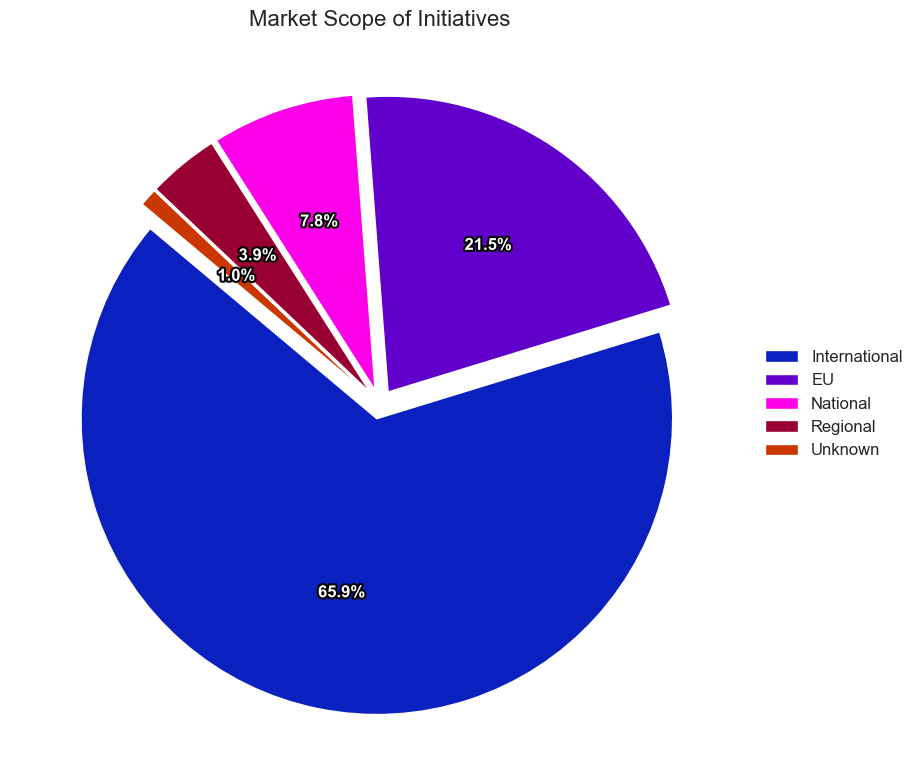
\includegraphics[width=0.7\textwidth]{figures/initiatives_market_scope.png}
  \caption{%
    \textit{Market Scope of Initiatives} 
  }
  \label{fig:initiatives_market_scope}
\end{figure}

A high-level indicator of each project’s target audience and regulatory environment is the market scope, that is, whether an initiative operates or aims to operate at a national, regional, EU, or international level. As illustrated in \Cref{fig:initiatives_market_scope}, the majority of the examined initiatives (approximately 66\%) describe themselves as international, while around 22\% are \ac{eu}-focused. A smaller fraction ($\sim$4\%) restrict their efforts to a single country (national scope), with only 1\% reported as “regional” (e.g., targeting multi-country clusters outside the \ac{eu} context). Notably, $\sim$8\% of initiatives do not specify a market scope at all. This distribution suggests that, even at this relatively early stage, many \ac{dpp} endeavors recognize the inherently global nature of supply chains and thus seek to address transnational interoperability challenges, an observation aligning with the multi-stakeholder, cross-border perspective emphasized previously in \Cref{cha:chapter_2}.

\begin{figure}[htbp]
  \centering
  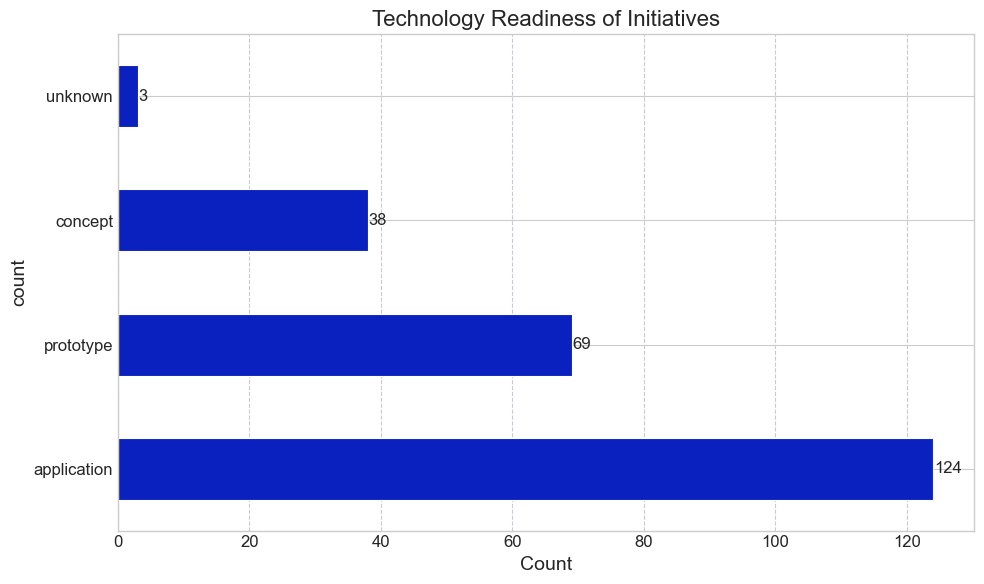
\includegraphics[width=\textwidth]{figures/initiatives_tech_readiness.png}
  \caption{%
    \textit{Technology Readiness of Initiatives} 
  }
  \label{fig:initiatives_tech_readiness}
\end{figure}

\Cref{fig:initiatives_tech_readiness} displays the distribution of initiatives by technology readiness level, categorized into concept, prototype, application, or unknown. A plurality (approximately 60\%) of the dataset falls under the application stage, implying that these projects claim some level of real-world implementation or near-market deployment. According to CIRPASS, the maturity level is determined based on observable activity in the industry, meaning that initiatives categorized at the application level have at the very least deployed a pilot solution within an industrial context. \autocite{CIRPASS.2024} Another significant portion ($\sim$34\%) remains at the prototype phase, highlighting ongoing experimentation and pilot testing in the \ac{dpp} domain. About 19\% are still conceptual, indicating that certain projects remain in the planning or proof-of-concept phase. It is also important to note that if a host organization leads multiple initiatives at different maturity levels, each initiative is counted separately in this analysis. Overall, these results reinforce the notion that many \ac{dpp} initiatives have advanced beyond mere theoretical discussions and are now exploring or refining practical solutions, albeit with varying degrees of maturity.

\begin{figure}[htbp]
  \centering
  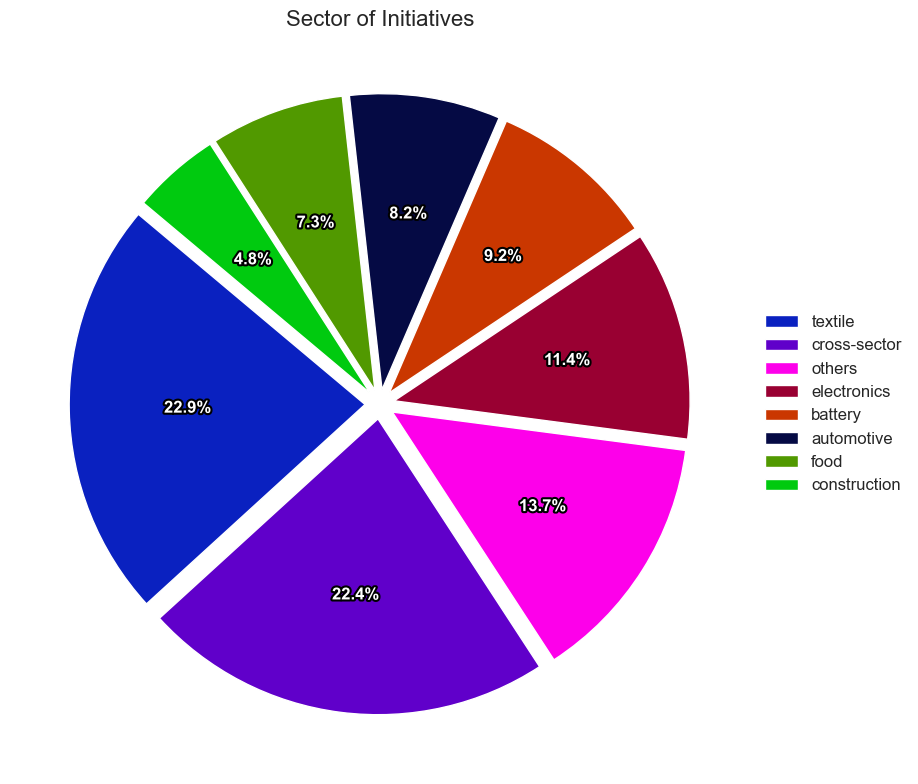
\includegraphics[width=0.7\textwidth]{figures/initiatives_sector.png}
  \caption{%
    \textit{Sector of Initiatives} 
  }
  \label{fig:initiatives_sector}
\end{figure}

In \Cref{fig:initiatives_sector}, a pie chart outlines the sector coverage of \ac{dpp} initiatives, demonstrating that the dataset spans a diverse range of industries. Textile and cross-sector projects collectively account for nearly half the sample (both around 22–23\%), reflecting the strong policy focus on textile sustainability (e.g., the \ac{eu} Strategy for Sustainable and Circular Textiles) and the broad applicability of \ac{dpp} concepts across multiple value chains. Electronics (9.2\%) and battery (7.3\%) are also notable, likely driven by emerging regulations on battery traceability and e-waste management (cf. \Cref{sec:regulatory_landscape}).

The presence of additional sectors such as automotive, food, and construction underscores the growing recognition that \ac{dpp} frameworks sooner or later have to be adapted to widely differing product categories, especially where traceability, compliance, or sustainability claims are paramount.

\begin{figure}[htbp]
  \centering
  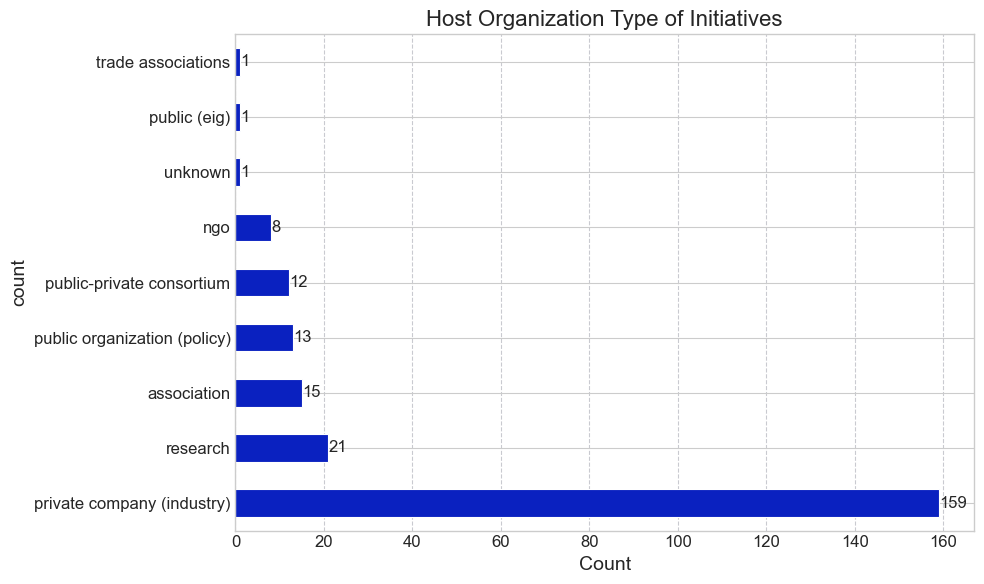
\includegraphics[width=\textwidth]{figures/initiatives_org_type.png}
  \caption{%
    \textit{Host Organization Type of Initiatives} 
  }
  \label{fig:initiatives_org_type}
\end{figure}

Turning to \Cref{fig:initiatives_org_type}, the host organization type reveals that an overwhelming majority (roughly 78\%) of these initiatives are led by private companies (industry). While associations, public bodies, and research institutions collectively appear in smaller proportions, their presence suggests a multi-faceted ecosystem in which industry-driven efforts coexist with policy-focused and academic collaborations. This distribution hints at a strong market pull for \ac{dpp} solutions, particularly among commercial entities seeking to differentiate via transparent supply chains or respond proactively to evolving regulatory mandates. Yet, the involvement of public-private consortia and research organizations underscores the need for cross-sectoral partnerships to address complex technical, legal, and societal challenges in implementing digital passports at scale.

\begin{figure}[H]
  \centering
  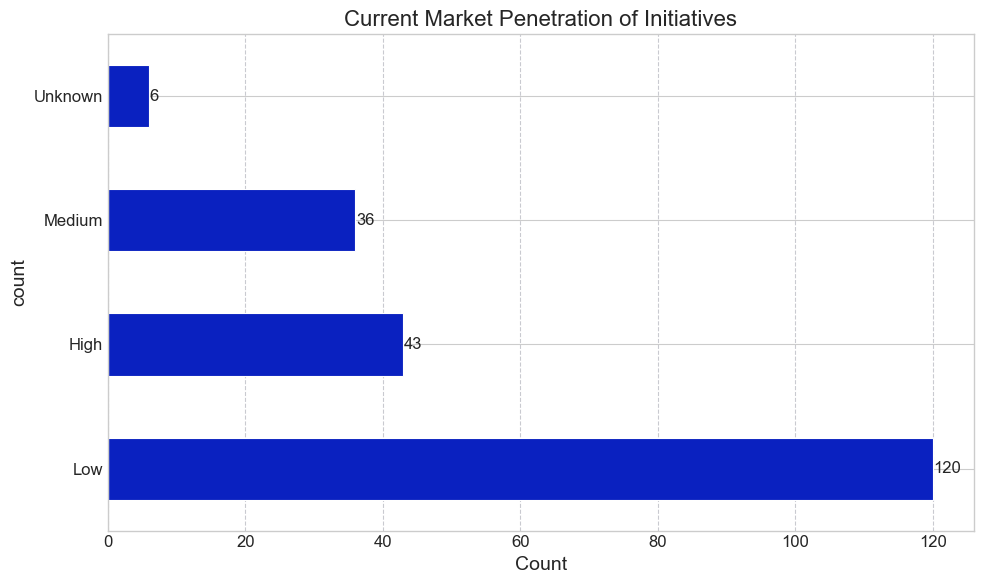
\includegraphics[width=0.8\textwidth]{figures/initiatives_market_penetration.png}
  \caption{%
    \textit{Current Market Penetration of Initiatives} 
  }
  \label{fig:initiatives_market_penetration}
\end{figure}

Beyond sectoral distribution and technology readiness, another critical dimension of \ac{dpp} initiatives lies in their market presence, revenue structures, and stakeholder focus. As shown in \Cref{fig:initiatives_market_penetration}, approximately 60\% of the analyzed initiatives report low market penetration, while only about 21\% claim high penetration, suggesting that most \ac{dpp} concepts have yet to achieve widespread commercial traction. This finding aligns with earlier observations about many projects remaining in prototype or pilot phases. Consequently, being in the application phase may simply indicate that an initiative has reached the minimum threshold for market deployment, such as a single implemented project or customer use case.

\begin{figure}[H]
  \centering
  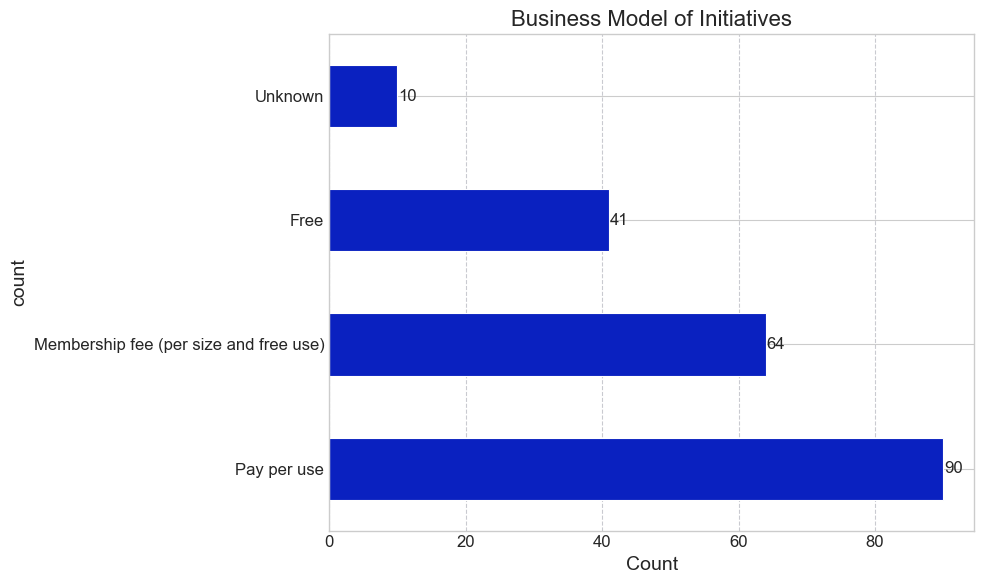
\includegraphics[width=0.8\textwidth]{figures/initiatives_buesiness_model.png}
  \caption{%
    \textit{Business Model of Initiatives} 
  }
  \label{fig:initiatives_buesiness_model}
\end{figure}

From a business model perspective \Cref{fig:initiatives_buesiness_model}, the majority ($\sim$44\%) of initiatives employ a “pay per use” scheme, charging their customers based on transaction volume or usage intensity. Another notable group ($\sim$31\%) relies on membership fees, often organized around tiered service levels. Meanwhile, a smaller cohort ($\sim$20\%) provides services free of charge, presumably leveraging alternative funding sources or indirect monetization. This variety of revenue approaches underscores the experimental stage of \ac{dpp} ecosystems, where providers continue to test which economic model fosters both long-term sustainability and user adoption.

% \begin{figure}[htbp]
%     \centering
%     \begin{minipage}{0.48\textwidth}
%         \centering
%         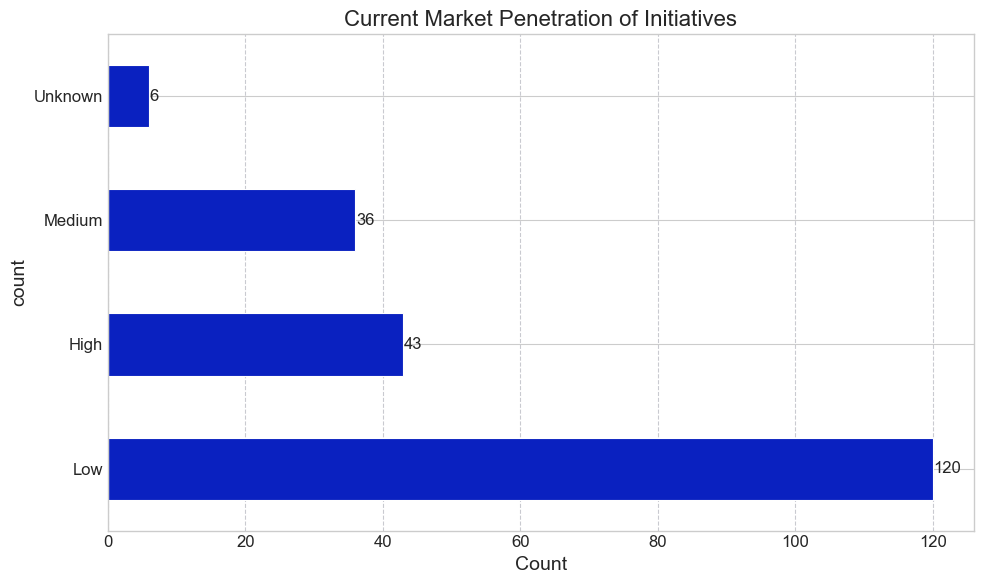
\includegraphics[width=\linewidth]{figures/initiatives_market_penetration.png}
%         \caption{\textit{Current Market Penetration of Initiatives}}
%         \label{fig:initiatives_market_penetration}
%     \end{minipage}
%     \hfill
%     \begin{minipage}{0.48\textwidth}
%         \centering
%         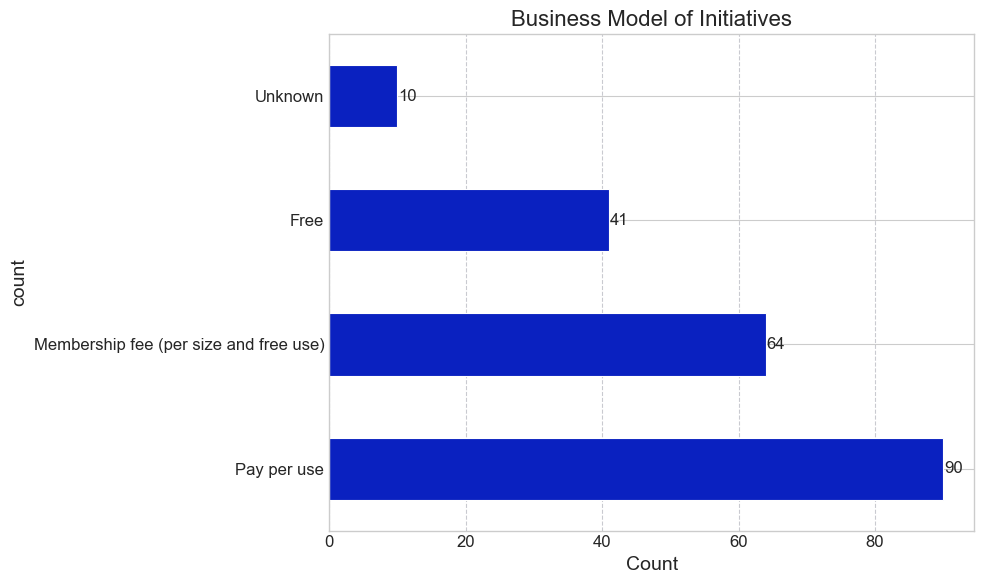
\includegraphics[width=\linewidth]{figures/initiatives_buesiness_model.png}
%         \caption{\textit{Business Model of Initiatives}}
%         \label{fig:initiatives_buesiness_model}
%     \end{minipage}
% \end{figure}

Finally, the co-occurrence heatmap that cross-tabulates target groups against industrial sectors  (\Cref{fig:initiatives_target_group_vs_sector}) illustrates how specific stakeholder groups intersect with various industries, revealing nuanced patterns of alignment and focus. For instance, distributors and retailers, manufacturers, and repair providers consistently appear in high counts across multiple sectors such as textiles and electronics, reflecting the \ac{dpp} solutions' focus on \acrlong{ce} models. Conversely, certain specialized roles (e.g., recycling material distributor or consumer protection associations) show stronger representation in heavily regulated or consumer-facing sectors. (e.g., batteries, food) This cross-tabulation reaffirms that \ac{dpp} initiatives not only demand diverse technical capabilities but also hinge on broad stakeholder involvement and collaborative networks among diverse stakeholders. Taken together, these findings reconfirm that while the \ac{dpp} market remains in a relatively early phase, its wide array of business models and stakeholder engagements indicates a dynamic, evolving ecosystem poised to adapt to regulatory shifts and user demands.

\begin{figure}[htbp]
  \centering
  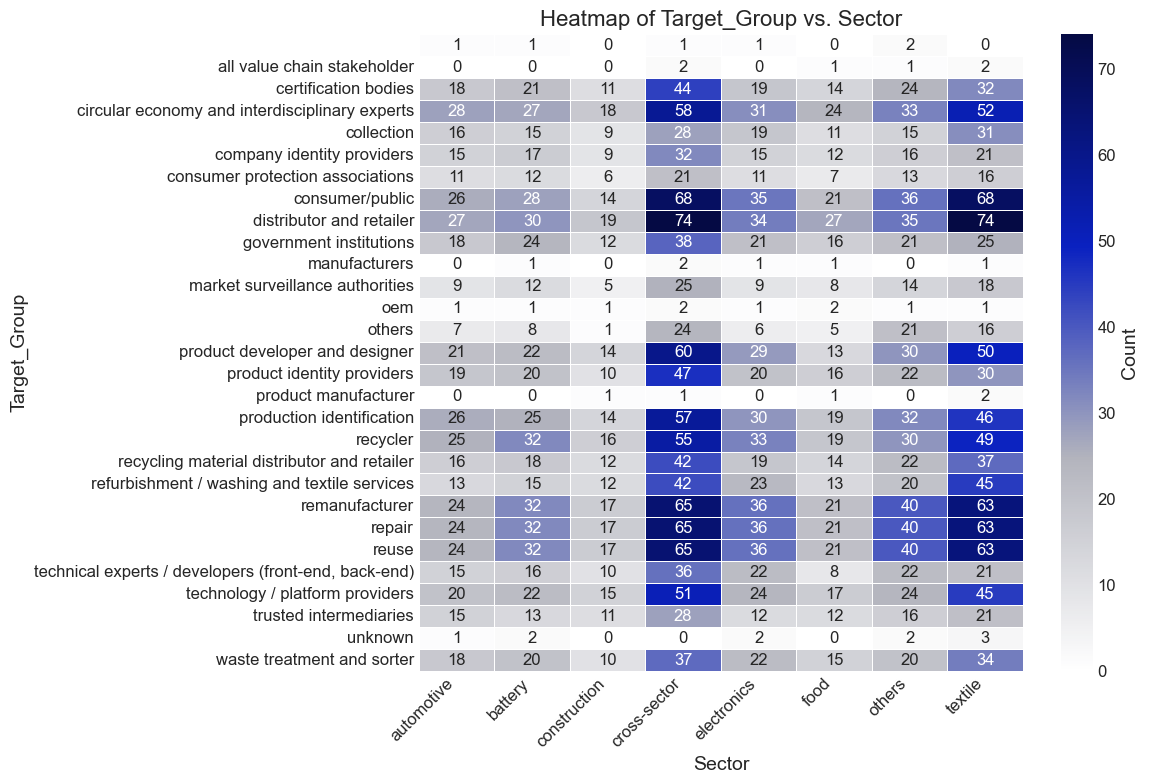
\includegraphics[width=\textwidth]{figures/initiatives_target_group_vs_sector.png}
  \caption{%
    \textit{Co-occurrence Heatmap of Target Groups and Sectors} 
  }
  \label{fig:initiatives_target_group_vs_sector}
\end{figure}

A core component of any \ac{dpp} system is how products are identified and how their corresponding data is minted and stored. The distribution of data carriers, the choice between centralized and decentralized ID minting, and the overarching data storage architecture are factors that together define the technical backbone of the \ac{dpp} initiatives.

\begin{figure}[H]
  \centering
  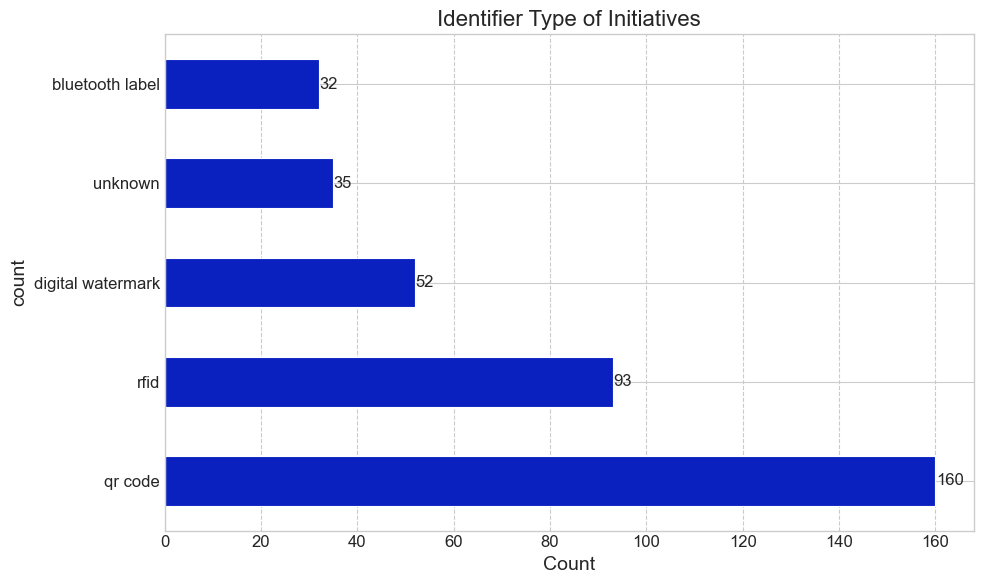
\includegraphics[width=0.8\textwidth]{figures/initiatives_data_carrier.png}
  \caption{%
    \textit{Data Carrier Type of Initiatives} 
  }
  \label{fig:initiatives_data_carrier}
\end{figure}

As shown in \Cref{fig:initiatives_data_carrier}, the most prevalent data carrier (or “identifier type”) across the dataset is \ac{qr} code, used by 160 initiatives. \ac{rfid} ranks second (93), followed by digital watermarks (52) and Bluetooth labels (32). Roughly 35 initiatives do not specify a carrier, recorded as “unknown.” This dominance of \ac{qr} codes may stem from their low cost, global familiarity, and ease of implementation, particularly for consumer-facing use cases (cf.\Cref{sec:dpp_concept_architecture} on Data Carriers). A smaller subset relies on digital watermarks or Bluetooth labels, indicating a willingness among some initiatives to experiment with emerging technologies that could offer enhanced security or offline detection capabilities.

\Cref{fig:initiatives_id_minting} and \Cref{fig:initiatives_storage_model} illustrate the ID minting and data storage choices, respectively, which further shape how \ac{dpp} solutions handle the generation, validation, and persistence of identifiers and lifecycle data. Notably, ID minting is split between decentralized (40.5\%) and centralized (42.0\%), with the remainder unknown. Likewise, data storage is predominantly decentralized (50.2\%) or centralized (37.1\%), with about 12.7\% unspecified. These proportions highlight a strong inclination toward distributed architectures, possibly reflecting concerns over data sovereignty, traceability, and tamper-resistance, attributes often cited in blockchain-based or peer-to-peer frameworks \autocite{Narayanan.2016}. However, the relatively balanced adoption of centralized models indicates that many initiatives still find conventional cloud or on-premise solutions suitable for \ac{dpp} implementation, particularly when logistical constraints discourage a fully decentralized approach.

\begin{figure}[htbp]
    \centering
    \begin{minipage}{0.48\textwidth}
        \centering
        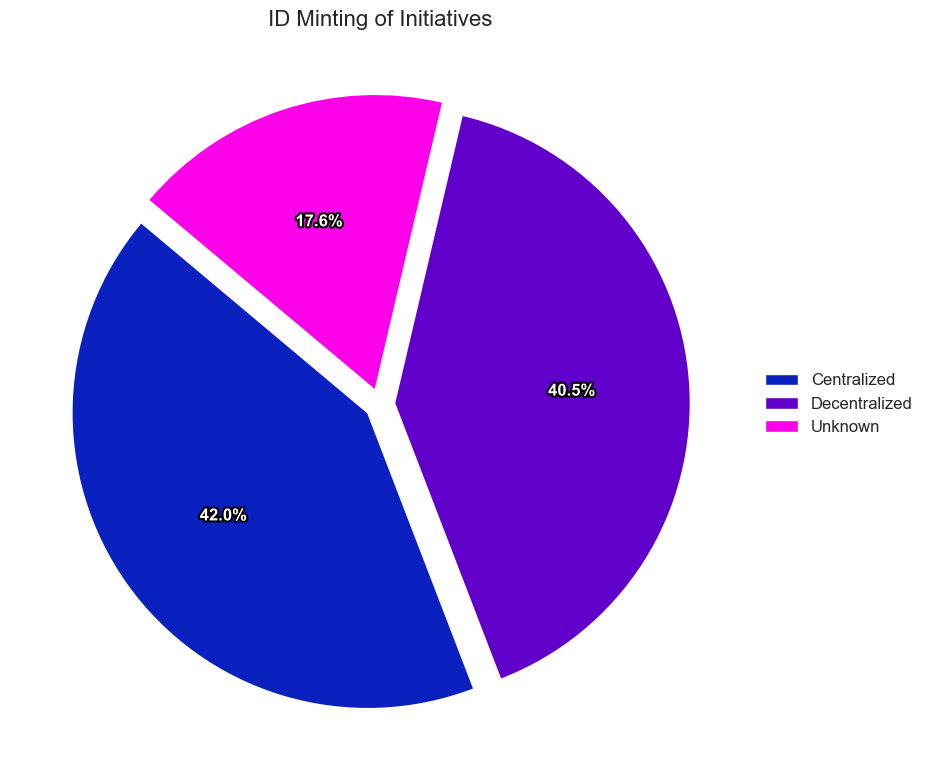
\includegraphics[width=\linewidth]{figures/initiatives_id_minting.png}
        \caption{\textit{ID Minting of Initiatives}}
        \label{fig:initiatives_id_minting}
    \end{minipage}
    \hfill
    \begin{minipage}{0.48\textwidth}
        \centering
        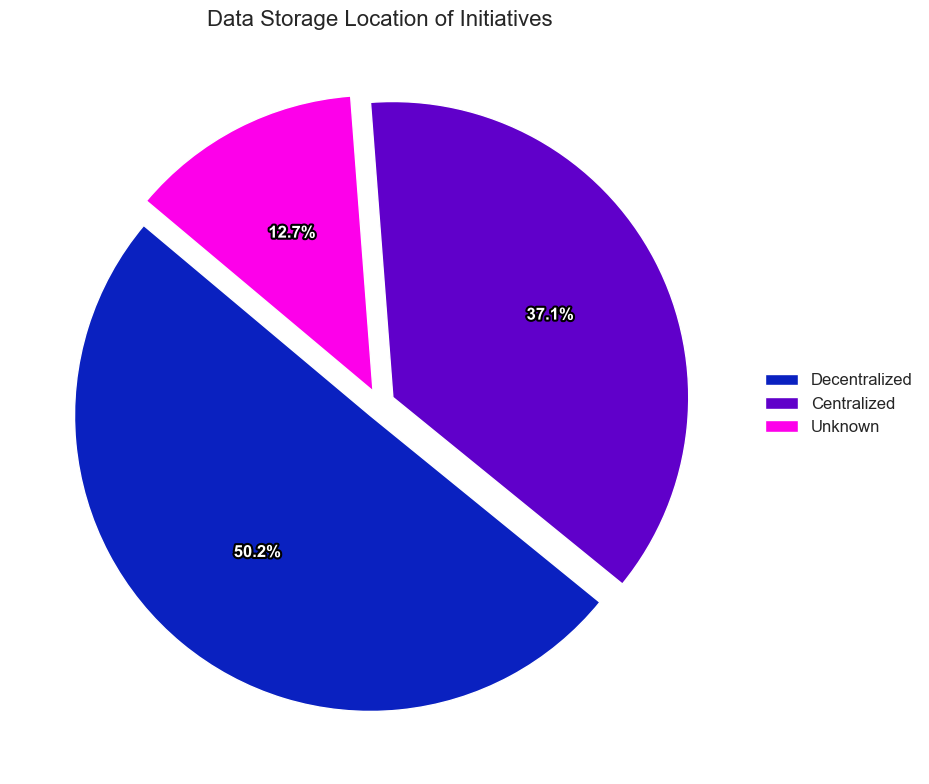
\includegraphics[width=\linewidth]{figures/initiatives_storage_model.png}
        \caption{\textit{Data Storage Model of Initiatives}}
        \label{fig:initiatives_storage_model}
    \end{minipage}
\end{figure}

A series of heatmaps reveal co-occurrence patterns among ID carriers, minting approaches, and data storage choices. For instance, the heatmap of "Identifier\_Type" vs. "ID\_Minting" 
(\Cref{fig:initiatives_data_carrier_vs_minting}) shows that \ac{qr} codes are widely employed regardless of whether ID minting is centralized or decentralized, suggesting that \ac{qr}-based solutions remain an easy, flexible option across governance models. By contrast, certain carriers (e.g., digital watermark) appear more concentrated in decentralized contexts, potentially indicating that advanced or less common carriers often pair with next-generation identity frameworks.

\begin{figure}[htbp]
  \centering
  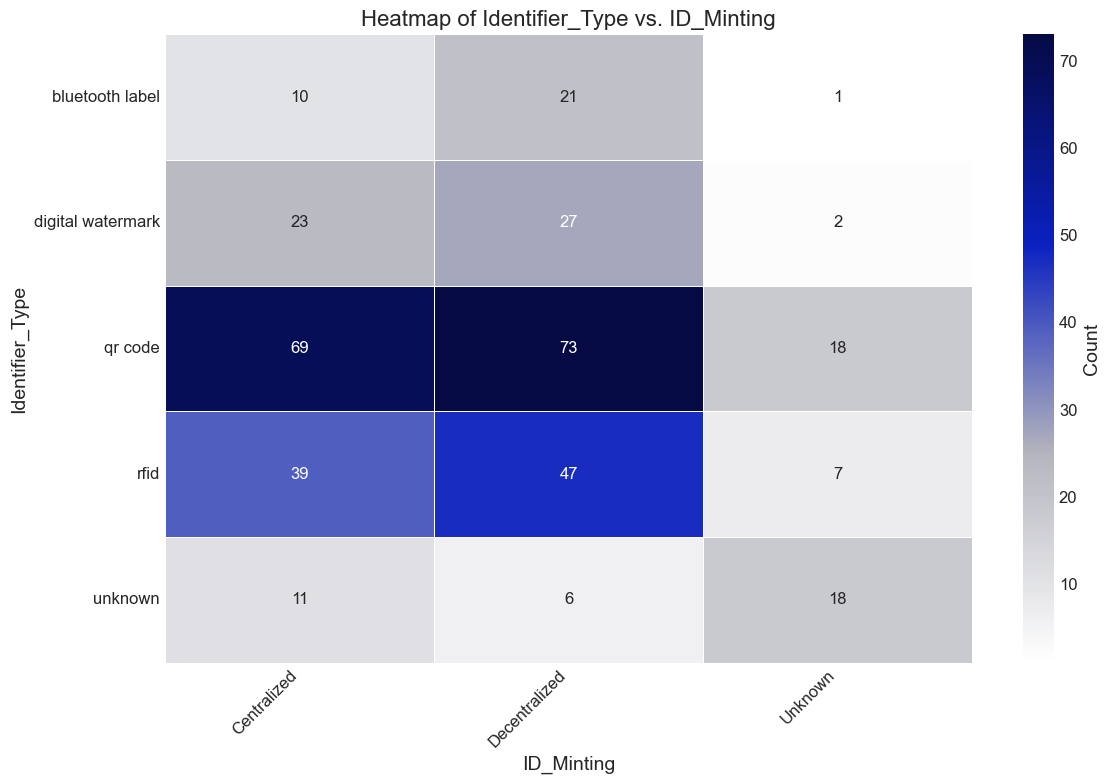
\includegraphics[width=0.7\textwidth]{figures/initiatives_data_carrier_vs_minting.png}
  \caption{%
    \textit{Co-occurrence Heatmap of Data Carriers Groups and ID Minting Approaches} 
  }
  \label{fig:initiatives_data_carrier_vs_minting}
\end{figure}

Similarly, the "ID\_Minting" vs. "Data\_Storage\_Location" (\Cref{fig:initiatives_minting_vs_storage}) cross-tabulation underscores that decentralized ID minting often pairs with decentralized storage, although a non-trivial fraction of initiatives adopt mixed approaches (e.g., decentralized minting but centralized data). This complexity signals a willingness to experiment with hybrid architectures, where product identities are minted on distributed ledgers, yet certain data elements remain in conventional cloud repositories for performance or governance reasons.

\begin{figure}[htbp]
  \centering
  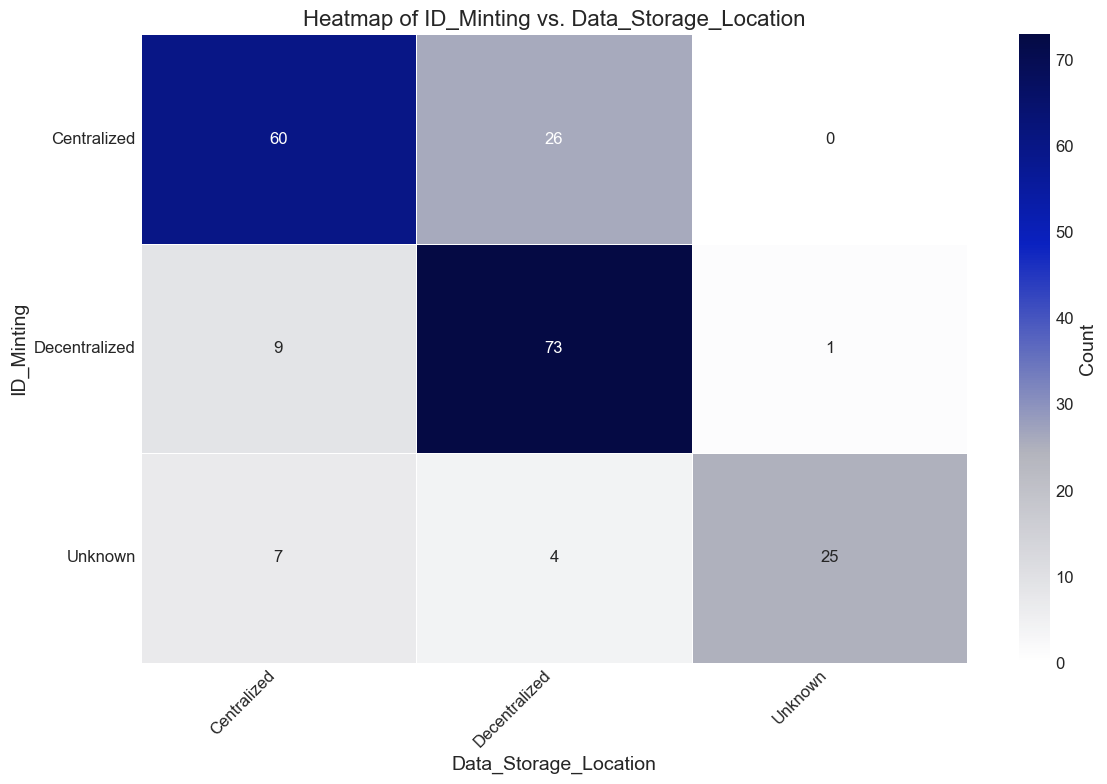
\includegraphics[width=0.7\textwidth]{figures/initiatives_minting_vs_storage.png}
  \caption{%
    \textit{Co-occurrence Heatmap of ID Minting Approaches and Storage Models} 
  }
  \label{fig:initiatives_minting_vs_storage}
\end{figure}

Next up, "Product\_ID\_Granularity" vs. "Data\_Storage\_Location" (\Cref{fig:initiatives_granularity_vs_storage}) confirms that while single-item tracking is prominent in decentralized storage (78) and batch-level identification is not uncommon, certain projects retain “production order” or “model”-level granularity in centralized databases. This spectrum of granularity underscores the diverse use cases \ac{dpp} solutions aim to address, from high-volume industrial scenarios requiring batch-level data to consumer-facing products requiring item-level details.

\begin{figure}[htbp]
  \centering
  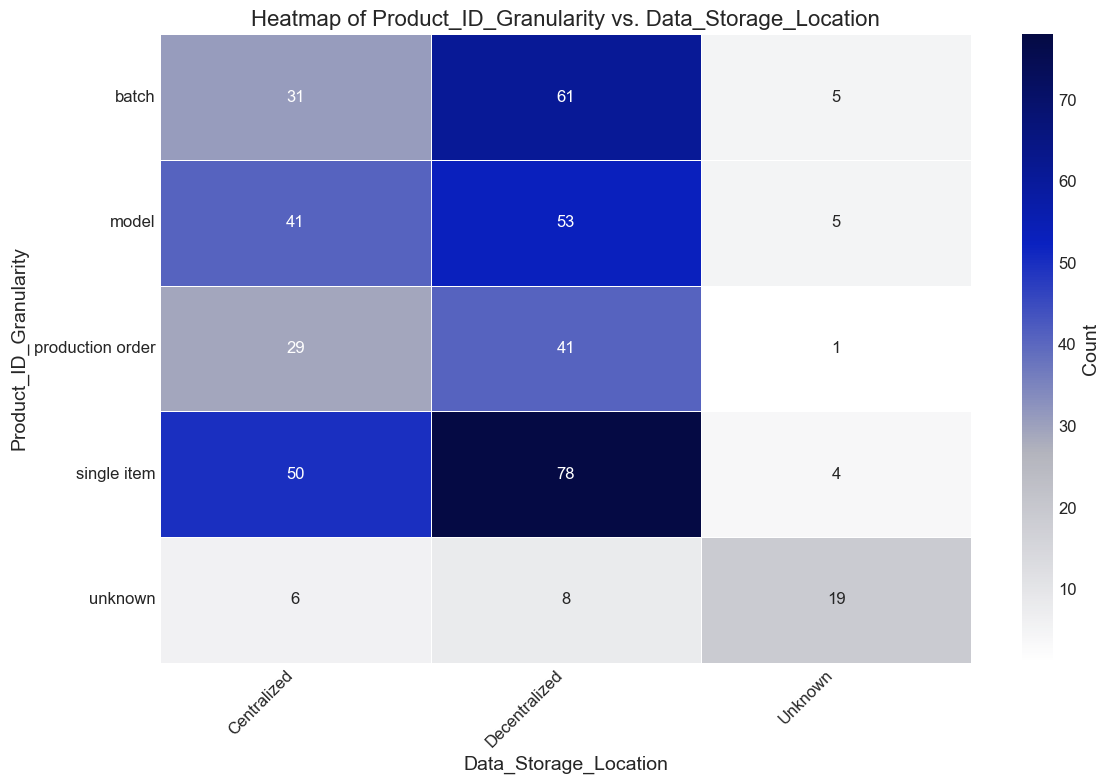
\includegraphics[width=0.7\textwidth]{figures/initiatives_granularity_vs_storage.png}
  \caption{%
    \textit{Co-occurrence Heatmap of Product ID Granularity and Storage Models} 
  }
  \label{fig:initiatives_granularity_vs_storage}
\end{figure}

\begin{figure}[htbp]
  \centering
  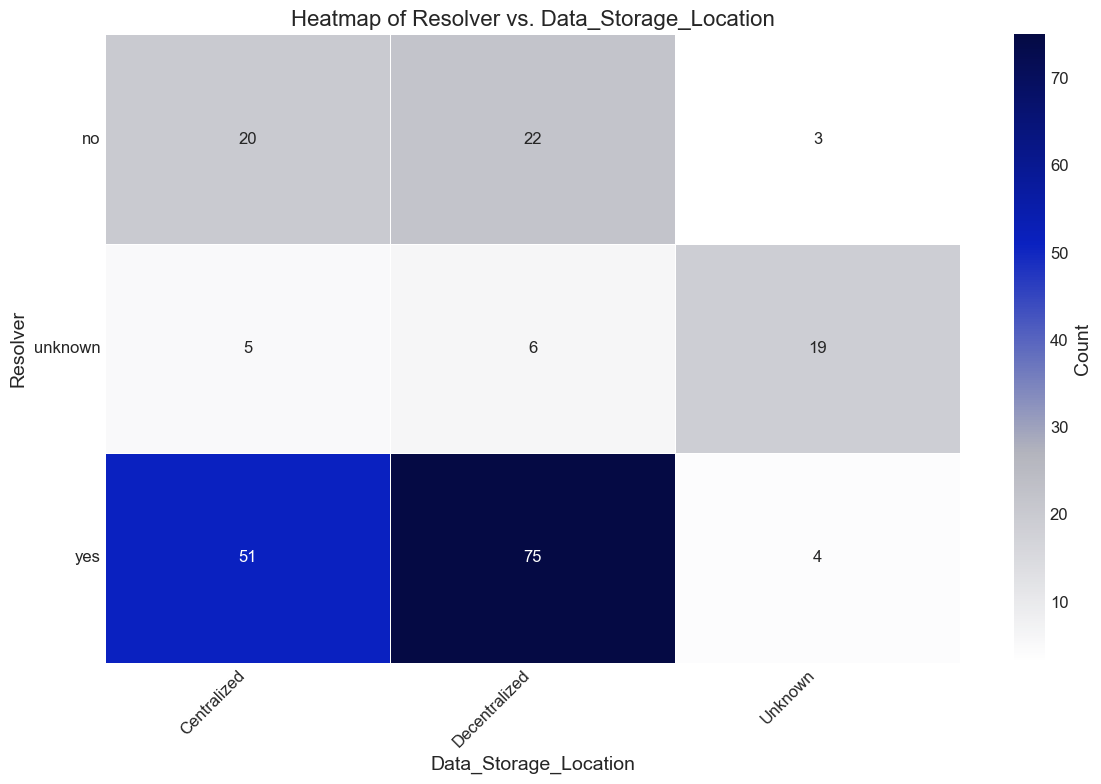
\includegraphics[width=0.7\textwidth]{figures/initiatives_resolver_vs_storage.png}
  \caption{%
    \textit{Co-occurrence Heatmap of Resolvers and Storage Models} 
  }
  \label{fig:initiatives_resolver_vs_storage}
\end{figure}

The "Resolver vs. Data\_Storage\_Location" heatmap (\Cref{fig:initiatives_resolver_vs_storage}) shows a strong correlation between decentralized storage and the presence of resolvers. Resolvers typically function as lookup services that map product identifiers to the correct data endpoint. In a decentralized context, resolvers may point to multiple distributed nodes or off-chain references, enhancing interoperability and redundancy \autocite{Liu.2022}. This synergy hints that many projects integrating decentralized architectures also invest in robust resolver frameworks to maintain seamless user experiences despite a fragmented storage landscape.

In order to capture the diverse technological interactions of \ac{dpp} solutions, a dedicated technology taxonomy was first established, mapping raw textual references, such as “qr code,” “rfid,” or “verifiable credential”, to broader categories (e.g., “data carrier,” “credentials,” “identity”). This grouping methodology transforms an otherwise fragmented arrays or unprocessed sentences into a manageable set of conceptual labels for co-occurrence analysis. \Cref{fig:initiatives_tech_cooccurrence} visualizes these categories and how often they appear together in the same initiative. The heatmap also reveals some less intuitive patterns, for instance, many initiatives adopt verifiable credentials (\ac{vc}) without relying on a distributed ledger, suggesting that cryptographic verification can be implemented in more centralized architectures. Similarly, identity-related solutions (e.g., self-sovereign identity) do not always coincide with blockchain, indicating that decentralized identification frameworks can be ledger-agnostic or prefer alternate cryptographic mechanisms. While some co-occurrences (such as privacy-enhancing technologies (PETs) or verifiable credentials (\ac{vc}) alongside blockchain) are unsurprising, given the push for tamper-resistant product data, the absence of such pairings in certain projects underscores the heterogeneity of \ac{dpp} technology stacks. \autocite{Narayanan.2016}

\begin{figure}[htbp]
  \centering
  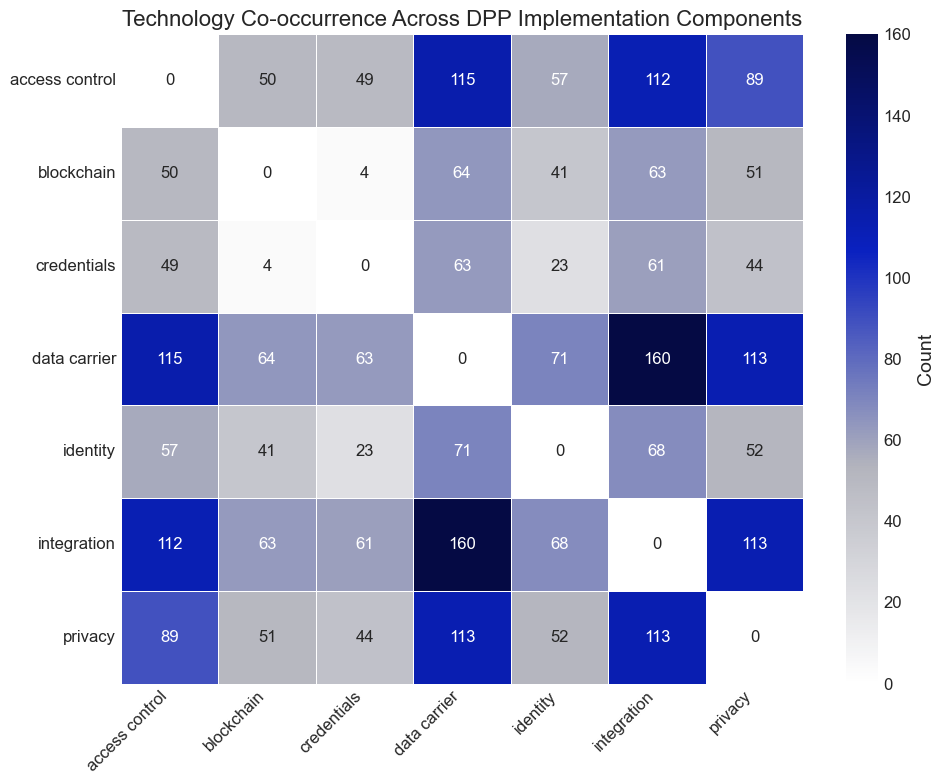
\includegraphics[width=0.8\textwidth]{figures/initiatives_tech_cooccurrence.png}
  \caption{%
    \textit{Technology Co-occurrence Across \ac{dpp} Implementation Components} 
  }
  \label{fig:initiatives_tech_cooccurrence}
\end{figure}

A complementary view is provided by the Technology Adoption by Implementation Maturity bar chart (\Cref{fig:initiatives_tech_adoption_by_maturity}), which cross-references the prevalence of technology categories (e.g., “access control,” “integration,” “blockchain”) with readiness levels (“concept,” “prototype,” “application”). Notably, data carrier technologies dominate across all stages, highlighting their fundamental role in linking physical products to digital records. Meanwhile, more complex components such as privacy and identity features tend to emerge more prominently in application-level initiatives, implying that robust security and identity management frameworks often mature after initial pilot phases have established baseline traceability.

\begin{figure}[htbp]
  \centering
  \vspace{-10pt}
  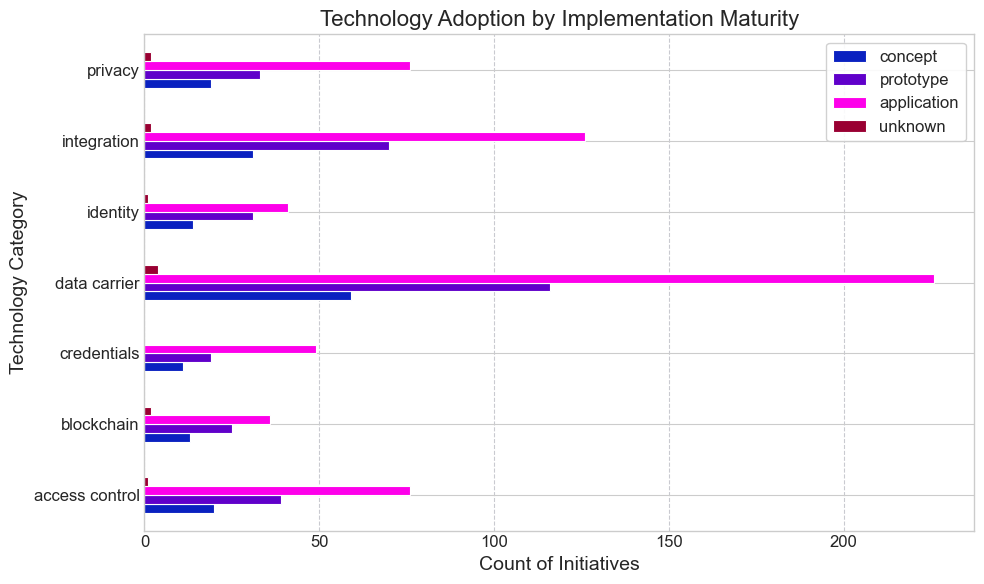
\includegraphics[width=\textwidth]{figures/initiatives_tech_adoption_by_maturity.png}
  \vspace{-10pt}
  \caption{%
    \textit{Technology Adoption by Implementation Maturity} 
  }
  \label{fig:initiatives_tech_adoption_by_maturity}
\end{figure}

Finally, the technology network graph (\Cref{fig:initiatives_tech_network}) offers a holistic, node-based representation of how these tools interconnect. Each node denotes a specific technology (e.g., “QR code,” “Blockchain,” “Verifiable Credentials,” “Role-Based Access”, "Privacy-Enhancing Technologies (PETs)", "Application Programming Interface (API)"), while edges signify co-occurrences within the same \ac{dpp} initiative. Node size reflects the frequency with which a technology appears across initiatives, while the distance between nodes is determined by their degree of co-occurrence, meaning that technologies frequently appearing together are positioned closer. Upon examination, several clusters become evident, with data carriers (\ac{qr} code, \ac{rfid}) at the center of many connections, and blockchain or smart contract solutions forming another influential cluster, often paired with credentials, privacy tools, or access control. This structure underlines the modular, integrative nature of contemporary \ac{dpp} systems, where physical product identifiers converge with cryptographic methods, semantic standards, and user-facing interfaces to build comprehensive, trustworthy product passports.

\begin{figure}[!ht]
  \centering
  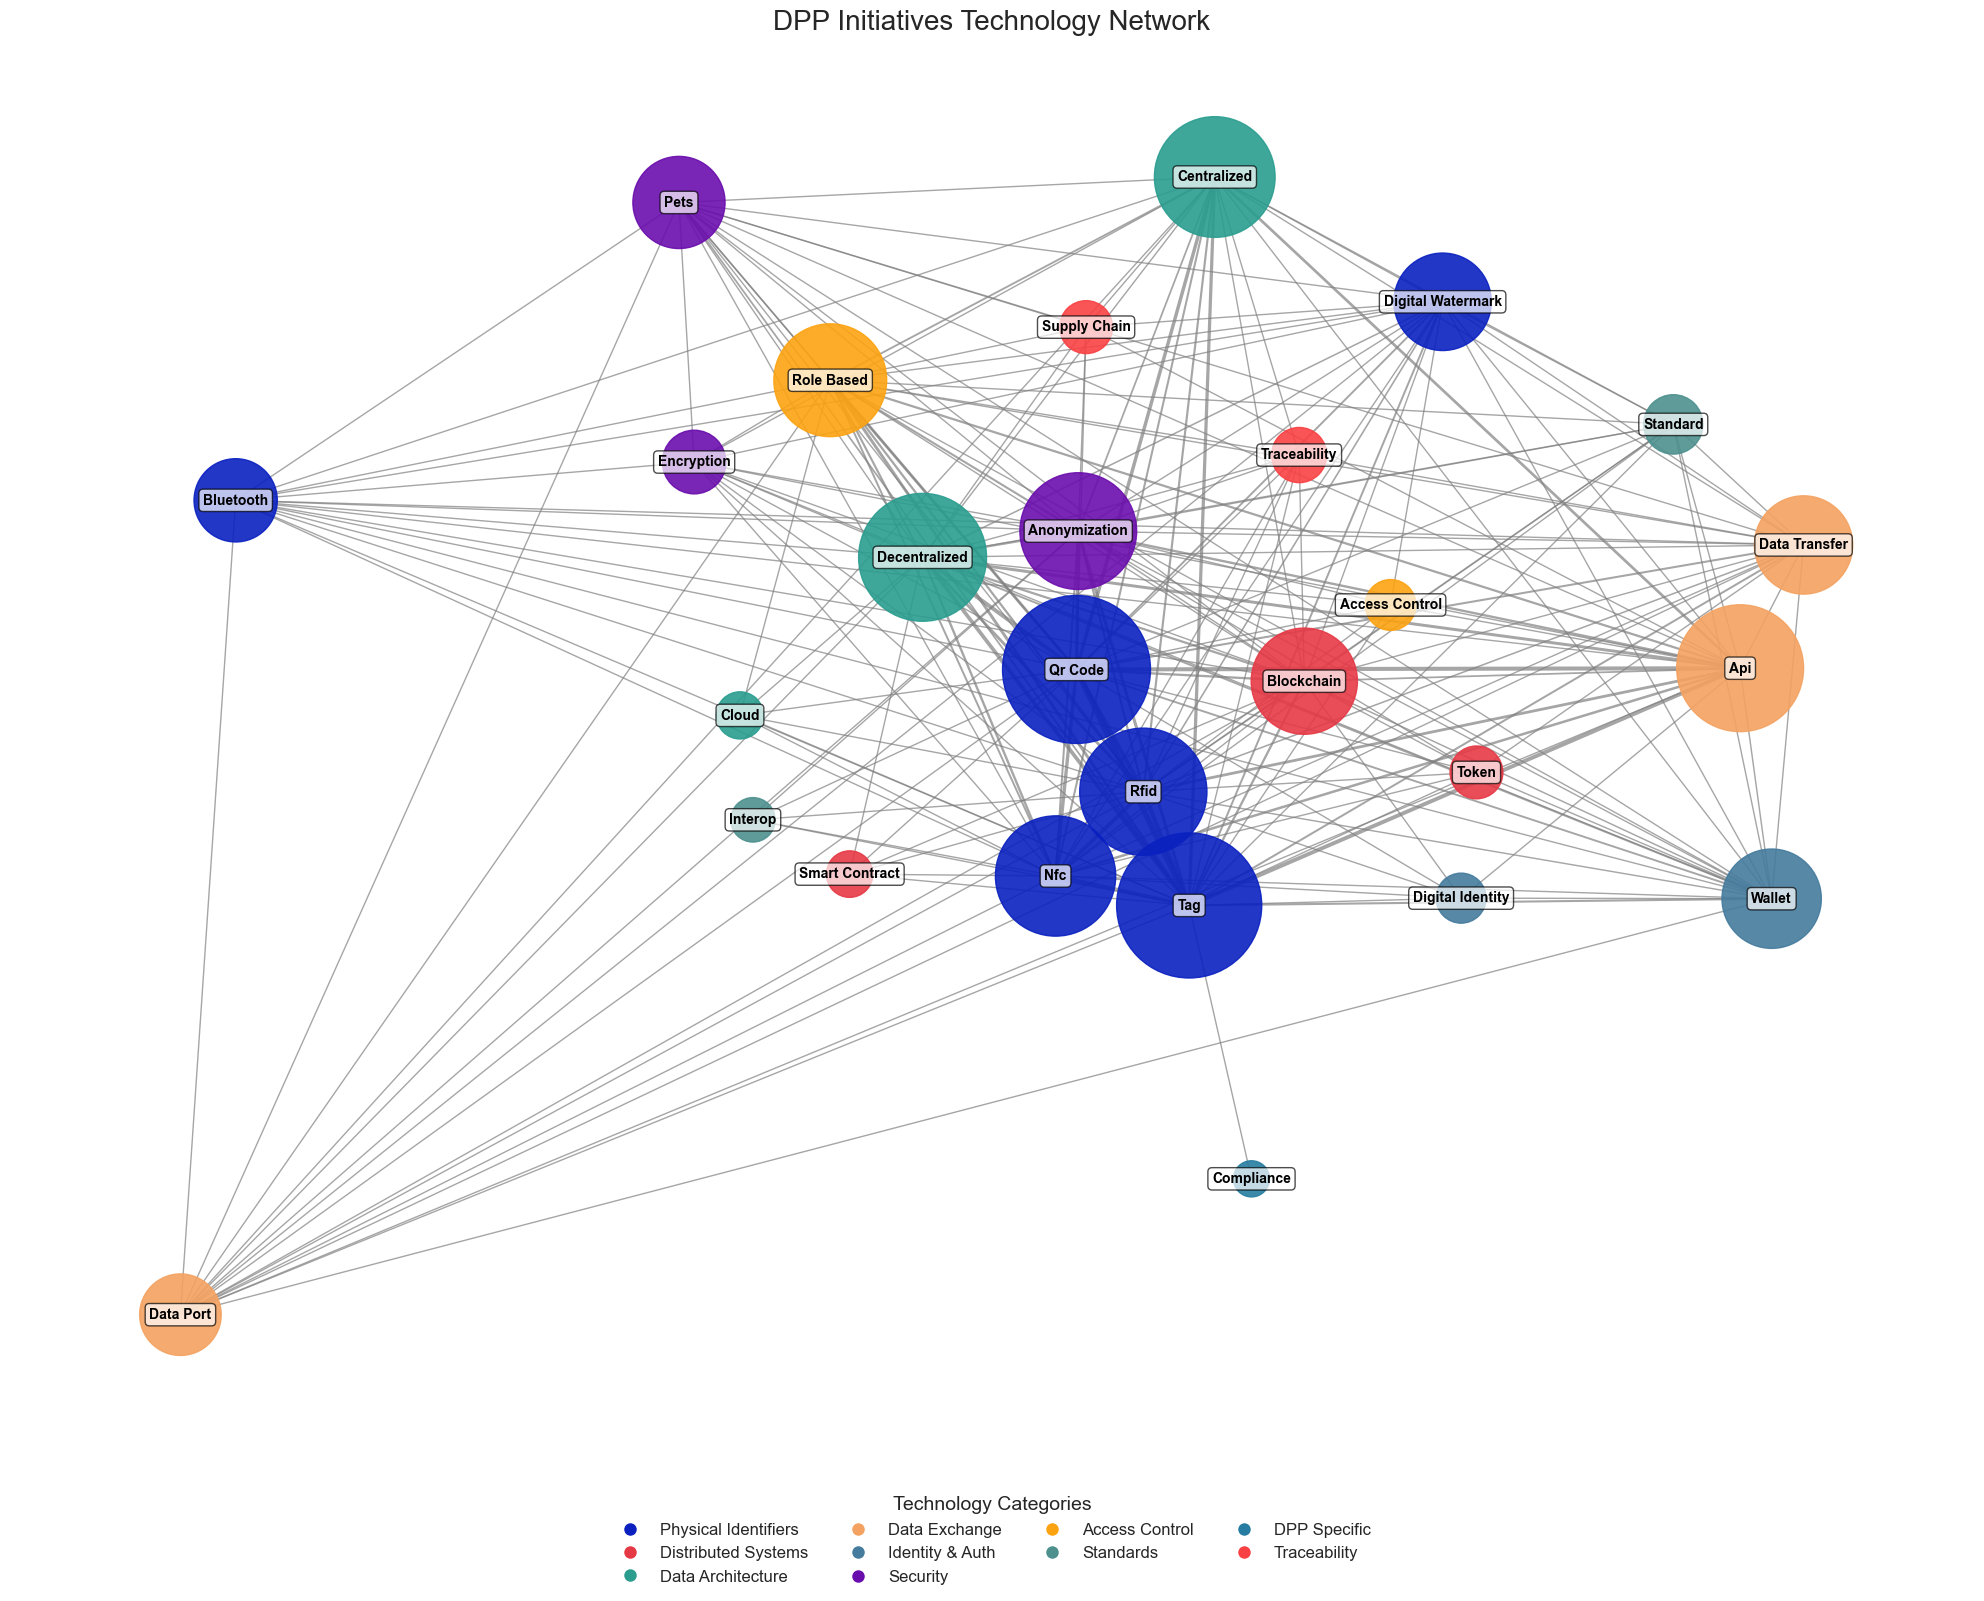
\includegraphics[width=\textwidth]{figures/initiatives_tech_network.png}
  \caption{%
    \textit{\ac{dpp} Initiatives Technology Network} 
  }
  \label{fig:initiatives_tech_network}
\end{figure}

Taken together, these visualizations show that although some \ac{dpp} initiatives still emphasize simpler, single-technology approaches, a growing number implement composite architectures that integrate data exchange protocols, identity management, and privacy-enhancing mechanisms.
